\documentclass{beamer}

\usepackage{fontspec}
\setmainfont[Ligatures=TeX]{Linux Libertine O}


\usepackage{tikz}

\usetikzlibrary{trees, arrows, shapes, automata, petri}
\usetikzlibrary{fit, calc, decorations}
\usetikzlibrary{decorations.pathreplacing}
\usetikzlibrary{decorations.pathmorphing}
\usetikzlibrary{positioning}
\usetikzlibrary{shadings, fadings, patterns}
%\usepackage{pgfbaselayers}
\pgfdeclarelayer{background}
\pgfdeclarelayer{foreground}
\pgfsetlayers{background,main,foreground}

% COLORS (Tango)
\definecolor{LightButter}{rgb}{0.98,0.91,0.31}
\definecolor{LightOrange}{rgb}{0.98,0.68,0.24}
\definecolor{LightChocolate}{rgb}{0.91,0.72,0.43}
\definecolor{LightChameleon}{rgb}{0.54,0.88,0.20}
\definecolor{LightSkyBlue}{rgb}{0.45,0.62,0.81}
\definecolor{LightPlum}{rgb}{0.68,0.50,0.66}
\definecolor{LightScarletRed}{rgb}{0.93,0.16,0.16}
\definecolor{Butter}{rgb}{0.93,0.86,0.25}
\definecolor{Orange}{rgb}{0.96,0.47,0.00}
\definecolor{Chocolate}{rgb}{0.75,0.49,0.07}
\definecolor{Chameleon}{rgb}{0.45,0.82,0.09}
\definecolor{SkyBlue}{rgb}{0.20,0.39,0.64}
\definecolor{Plum}{rgb}{0.46,0.31,0.48}
\definecolor{ScarletRed}{rgb}{0.80,0.00,0.00}
\definecolor{DarkButter}{rgb}{0.77,0.62,0.00}
\definecolor{DarkOrange}{rgb}{0.80,0.36,0.00}
\definecolor{DarkChocolate}{rgb}{0.56,0.35,0.01}
\definecolor{DarkChameleon}{rgb}{0.30,0.60,0.02}
\definecolor{DarkSkyBlue}{rgb}{0.12,0.29,0.53}
\definecolor{DarkPlum}{rgb}{0.36,0.21,0.40}
\definecolor{DarkScarletRed}{rgb}{0.64,0.00,0.00}
\definecolor{Aluminium1}{rgb}{0.93,0.93,0.92}
\definecolor{Aluminium2}{rgb}{0.82,0.84,0.81}
\definecolor{Aluminium3}{rgb}{0.73,0.74,0.71}
\definecolor{Aluminium4}{rgb}{0.53,0.54,0.52}
\definecolor{Aluminium5}{rgb}{0.33,0.34,0.32}
\definecolor{Aluminium6}{rgb}{0.18,0.20,0.21}

\setbeamercolor{alerted text}{fg=DarkScarletRed}
\setbeamercolor{background canvas}{bg=white}
\setbeamercolor{block body alerted}{bg=normal text.bg!90!black}
\setbeamercolor{block body}{bg=normal text.bg!90!black}
\setbeamercolor{block body example}{bg=normal text.bg!90!black}
\setbeamercolor{block title alerted}{use={normal text,alerted text},fg=alerted text.fg!75!normal text.fg,bg=normal text.bg!75!black}
\setbeamercolor{block title}{bg=Plum,fg=Aluminium1}
\setbeamercolor{block title example}{use={normal text,example text},fg=example text.fg!75!normal text.fg,bg=normal text.bg!75!black}
\setbeamercolor{fine separation line}{}
\setbeamercolor{frametitle}{fg=Aluminium1,bg=LightPlum}
\setbeamercolor{item projected}{fg=Aluminium1,parent=palette primary}
\setbeamercolor{normal text}{bg=white,fg=Aluminium6}
\setbeamercolor{palette sidebar primary}{use=normal text,fg=normal text.fg}
\setbeamercolor{palette sidebar quaternary}{use=structure,fg=structure.fg}
\setbeamercolor{palette sidebar secondary}{use=structure,fg=structure.fg}
\setbeamercolor{palette sidebar tertiary}{use=normal text,fg=normal text.fg}
\setbeamercolor{section in sidebar}{fg=Chameleon}
\setbeamercolor{section in sidebar shaded}{fg=Chameleon}
\setbeamercolor{separation line}{}
\setbeamercolor{sidebar}{bg=Chameleon}
\setbeamercolor{sidebar}{parent=palette primary}
\setbeamercolor{structure}{bg=Aluminium1,fg=Plum}
\setbeamercolor{subsection in sidebar}{fg=Chameleon}
\setbeamercolor{subsection in sidebar shaded}{fg=Chameleon}
\setbeamercolor{title}{fg=Aluminium1,bg=LightPlum}
\setbeamercolor{titlelike}{fg=Aluminium1}


\tikzset{
	locnode base/.style = {
		rectangle,
		rounded corners = 2pt,
		text centered,
		minimum height = 5mm,
		minimum width = 10mm,
        bottom color = Aluminium1
	},
    locnode grey/.style = {
        locnode base,
		draw = Aluminium6,
		top color = Aluminium1,
		bottom color = Aluminium2
    },
    locnode/.style = {
        locnode grey
    },
	locnode orange/.style = {
        locnode base,
        draw = DarkOrange,
		top color = LightOrange,
		bottom color = Orange
	},
	locnode green/.style = {
        locnode base,
        draw = DarkChameleon,
		top color = Aluminium1,
		bottom color = Chameleon
	},
	locnode red/.style = {
        locnode base,
        draw = DarkScarletRed,
		top color = Aluminium1,
		bottom color = LightScarletRed
	},
	locnode plum/.style = {
        locnode base,
        draw = DarkPlum,
		top color = Aluminium1,
		bottom color = LightPlum
	},
	locnode blue/.style = {
        locnode base,
        draw = DarkSkyBlue,
		top color = Aluminium1,
		bottom color = LightSkyBlue
	},
	locnode brown/.style = {
        locnode base,
        draw = DarkChocolate,
		top color = Aluminium1,
		bottom color = LightChocolate
	},
	locnode yellow/.style = {
        locnode base,
        draw = DarkButter,
		top color = Aluminium1, % LightButter,
		bottom color = Butter
	}
}


\usepackage{beamerthemesplit}
\usepackage{wasysym}

\usetheme{Copenhagen}
%\usecolortheme{crane}
%\useoutertheme{infolines}
% COLORS (Tango)
\definecolor{LightButter}{rgb}{0.98,0.91,0.31}
\definecolor{LightOrange}{rgb}{0.98,0.68,0.24}
\definecolor{LightChocolate}{rgb}{0.91,0.72,0.43}
\definecolor{LightChameleon}{rgb}{0.54,0.88,0.20}
\definecolor{LightSkyBlue}{rgb}{0.45,0.62,0.81}
\definecolor{LightPlum}{rgb}{0.68,0.50,0.66}
\definecolor{LightScarletRed}{rgb}{0.93,0.16,0.16}
\definecolor{Butter}{rgb}{0.93,0.86,0.25}
\definecolor{Orange}{rgb}{0.96,0.47,0.00}
\definecolor{Chocolate}{rgb}{0.75,0.49,0.07}
\definecolor{Chameleon}{rgb}{0.45,0.82,0.09}
\definecolor{SkyBlue}{rgb}{0.20,0.39,0.64}
\definecolor{Plum}{rgb}{0.46,0.31,0.48}
\definecolor{ScarletRed}{rgb}{0.80,0.00,0.00}
\definecolor{DarkButter}{rgb}{0.77,0.62,0.00}
\definecolor{DarkOrange}{rgb}{0.80,0.36,0.00}
\definecolor{DarkChocolate}{rgb}{0.56,0.35,0.01}
\definecolor{DarkChameleon}{rgb}{0.30,0.60,0.02}
\definecolor{DarkSkyBlue}{rgb}{0.12,0.29,0.53}
\definecolor{DarkPlum}{rgb}{0.36,0.21,0.40}
\definecolor{DarkScarletRed}{rgb}{0.64,0.00,0.00}
\definecolor{Aluminium1}{rgb}{0.93,0.93,0.92}
\definecolor{Aluminium2}{rgb}{0.82,0.84,0.81}
\definecolor{Aluminium3}{rgb}{0.73,0.74,0.71}
\definecolor{Aluminium4}{rgb}{0.53,0.54,0.52}
\definecolor{Aluminium5}{rgb}{0.33,0.34,0.32}
\definecolor{Aluminium6}{rgb}{0.18,0.20,0.21}

\setbeamercolor{alerted text}{fg=DarkScarletRed}
\setbeamercolor{background canvas}{bg=white}
\setbeamercolor{block body alerted}{bg=normal text.bg!90!black}
\setbeamercolor{block body}{bg=normal text.bg!90!black}
\setbeamercolor{block body example}{bg=normal text.bg!90!black}
\setbeamercolor{block title alerted}{use={normal text,alerted text},fg=alerted text.fg!75!normal text.fg,bg=normal text.bg!75!black}
\setbeamercolor{block title}{bg=Plum,fg=Aluminium1}
\setbeamercolor{block title example}{use={normal text,example text},fg=example text.fg!75!normal text.fg,bg=normal text.bg!75!black}
\setbeamercolor{fine separation line}{}
\setbeamercolor{frametitle}{fg=Aluminium1,bg=LightPlum}
\setbeamercolor{item projected}{fg=Aluminium1,parent=palette primary}
\setbeamercolor{normal text}{bg=white,fg=Aluminium6}
\setbeamercolor{palette sidebar primary}{use=normal text,fg=normal text.fg}
\setbeamercolor{palette sidebar quaternary}{use=structure,fg=structure.fg}
\setbeamercolor{palette sidebar secondary}{use=structure,fg=structure.fg}
\setbeamercolor{palette sidebar tertiary}{use=normal text,fg=normal text.fg}
\setbeamercolor{section in sidebar}{fg=Chameleon}
\setbeamercolor{section in sidebar shaded}{fg=Chameleon}
\setbeamercolor{separation line}{}
\setbeamercolor{sidebar}{bg=Chameleon}
\setbeamercolor{sidebar}{parent=palette primary}
\setbeamercolor{structure}{bg=Aluminium1,fg=Plum}
\setbeamercolor{subsection in sidebar}{fg=Chameleon}
\setbeamercolor{subsection in sidebar shaded}{fg=Chameleon}
\setbeamercolor{title}{fg=Aluminium1,bg=LightPlum}
\setbeamercolor{titlelike}{fg=Aluminium1}


\tikzset{
	locnode base/.style = {
		rectangle,
		rounded corners = 2pt,
		text centered,
		minimum height = 5mm,
		minimum width = 10mm,
        bottom color = Aluminium1
	},
    locnode grey/.style = {
        locnode base,
		draw = Aluminium6,
		top color = Aluminium1,
		bottom color = Aluminium2
    },
    locnode/.style = {
        locnode grey
    },
	locnode orange/.style = {
        locnode base,
        draw = DarkOrange,
		top color = LightOrange,
		bottom color = Orange
	},
	locnode green/.style = {
        locnode base,
        draw = DarkChameleon,
		top color = Aluminium1,
		bottom color = Chameleon
	},
	locnode red/.style = {
        locnode base,
        draw = DarkScarletRed,
		top color = Aluminium1,
		bottom color = LightScarletRed
	},
	locnode plum/.style = {
        locnode base,
        draw = DarkPlum,
		top color = Aluminium1,
		bottom color = LightPlum
	},
	locnode blue/.style = {
        locnode base,
        draw = DarkSkyBlue,
		top color = Aluminium1,
		bottom color = LightSkyBlue
	},
	locnode brown/.style = {
        locnode base,
        draw = DarkChocolate,
		top color = Aluminium1,
		bottom color = LightChocolate
	},
	locnode yellow/.style = {
        locnode base,
        draw = DarkButter,
		top color = Aluminium1, % LightButter,
		bottom color = Butter
	}
}


\setbeamertemplate{headline}{}
\setbeamertemplate{footline}{}

\setbeamertemplate{navigation symbols}{%
    %\insertdocnavigationsymbol
    \ifnum\theframenumber=0\relax\else%
        \normalsize\textcolor{DarkPlum}{\insertframenumber}%/\inserttotalframenumber}
    \fi%
    %\quad
}

\makeatletter
%\sectionframe[]{}
% no star: section name (facultative, if not specified, it is the second argument), the huge text written on the slide.
% one star: no section defined, the argument is the huge text.
% two stars: no section defined, the arguments are the huge text and some text to be written afterwards.
% I guess {\sectionframe}*: a if no stars, but with an additional argument, with is the text written afterwards.
\newcommand\sectionframe@star@add[2]{
    \begin{frame}
        \begin{center}
            \Huge \textcolor{Plum}{#1}
        \end{center}
        #2
    \end{frame}
}
\newcommand\sectionframe@unstar@add[3][]{
    \ifempty{#1}{\section{#2}}{\section{#1}}
    \sectionframe@star@add{#2}{#3}
}
\newcommand\sectionframe@star@base[1]{\sectionframe@star@add{#1}{}}
\newcommand\sectionframe@unstar@base[2][]{\sectionframe@unstar@add[#1]{#2}{}}
\newcommand\sectionframe@star{\@ifstar\sectionframe@star@add\sectionframe@star@base}
\newcommand\sectionframe@unstar{\@ifstar\sectionframe@unstar@add\sectionframe@unstar@base}
\newcommand\sectionframe{\@ifstar\sectionframe@star\sectionframe@unstar}
\makeatother

\newcommand<>\Alt[2]{{%
        \sbox0{$\displaystyle #1$}%
        \sbox1{$\displaystyle #2$}%
        \alt#3%
        {\rlap{\usebox0}\vphantom{\usebox1}\hphantom{\ifnum\wd0>\wd1 \usebox0\else\usebox1\fi}}%
        {\rlap{\usebox1}\vphantom{\usebox0}\hphantom{\ifnum\wd0>\wd1 \usebox0\else\usebox1\fi}}%
}}

\makeatletter
\newcommand\bsphere[2][-.65ex]{%
    \raisebox{#1}{%
    \begin{pgfpicture}[-1ex]{-.65ex}{1ex}{1ex}%
       \usebeamercolor[fg]{item projected}%
       {\pgftransformscale{1.75}\pgftext{\normalsize\pgfuseshading{bigsphere}}}%
       {\pgftransformshift{\pgfpoint{0pt}{.5pt}}%
           \pgftext{\usebeamerfont*{item projected}%
               \usebeamercolor[fg]{item projected}%
               #2%
           }%
       }%
    \end{pgfpicture}%
   }%
}
\makeatother

\newcommand\provedincoq[1]{%
    \vspace{-6.5mm}%
    \hfill%
    \parbox[b][0pt][b]{2cm}{%
        \hfill%
        \ifempty{#1}{%
            
\includegraphics[height = 8mm]{images/logo_tampon_3d.png}%
        }{%
            ~\vspace{-2mm}%
            \anchor{#1}{%
                
\includegraphics[height = 8mm]{images/logo_tampon_3d.png}%
            }%
            \hspace{-4mm}%
        }%
        \hspace{1mm}~%
    }%
    \vspace{4mm}%
}

\newenvironment{variableblock}[3]{%
    \setbeamercolor{block body}{#2}
    \setbeamercolor{block title}{#3}
          \begin{block}{#1}}{\end{block}}



\newcommand\ifempty[3]{\expandafter\ifstrempty{#1}{#2}{#3}}
\newcommand\ifnempty[2]{\expandafter\ifstrempty{#1}{}{#2}}
\newcommand\defaultempty[2]{\expandafter\ifstrempty{#1}{#2}{#1}}
\newcommand\ignore[1]{}

\usepackage[langlinenos,cache,newfloat]{minted}

\setminted{encoding=utf8}

\makeatletter
\newcommand{\minted@def@optcl@switch@simple}[2]{%
  \define@booleankey{minted@opt@g}{#1}%
    {\minted@addto@optlistcl{\minted@optlistcl@g}{#2}%
      \@namedef{minted@opt@g:#1}{true}}
    {\minted@addto@optlistcl{\minted@optlistcl@g}{}%
      \@namedef{minted@opt@g:#1}{false}}
  \define@booleankey{minted@opt@g@i}{#1}%
    {\minted@addto@optlistcl{\minted@optlistcl@g@i}{#2}%
      \@namedef{minted@opt@g@i:#1}{true}}
    {\minted@addto@optlistcl{\minted@optlistcl@g@i}{}%
      \@namedef{minted@opt@g@i:#1}{false}}
  \define@booleankey{minted@opt@lang}{#1}%
    {\minted@addto@optlistcl@lang{minted@optlistcl@lang\minted@lang}{#2}%
      \@namedef{minted@opt@lang\minted@lang:#1}{true}}
    {\minted@addto@optlistcl@lang{minted@optlistcl@lang\minted@lang}{}%
      \@namedef{minted@opt@lang\minted@lang:#1}{false}}
  \define@booleankey{minted@opt@lang@i}{#1}%
    {\minted@addto@optlistcl@lang{minted@optlistcl@lang\minted@lang @i}{#2}%
      \@namedef{minted@opt@lang\minted@lang @i:#1}{true}}
    {\minted@addto@optlistcl@lang{minted@optlistcl@lang\minted@lang @i}{}%
      \@namedef{minted@opt@lang\minted@lang @i:#1}{false}}
  \define@booleankey{minted@opt@cmd}{#1}%
      {\minted@addto@optlistcl{\minted@optlistcl@cmd}{#2}%
        \@namedef{minted@opt@cmd:#1}{true}}
      {\minted@addto@optlistcl{\minted@optlistcl@cmd}{}%
        \@namedef{minted@opt@cmd:#1}{false}}
}
% \minted@def@optcl@switch@simple{kwrename}{-F kwrenamefilter}
\makeatother

\usepackage{tcolorbox}

\tcbuselibrary{minted, skins}

\tcbset{programbox/.style = {
        enhanced,
        colback = LightPlum!10,
        colframe = DarkPlum,
        left = 1mm,
        listing only,
        listing engine = minted
    }
}

% Definition of programming languages used in the document.
\makeatletter
\newcommand\makenewlistings@aux[2]{
    \expandafter\newtcblisting{#2codenoescape}[1][]{
        programbox,
        listing only,
        minted language = #1,
        minted options= {
            % kwrename,
            linenos = true,
            fontsize = \small,
            ##1}
    }
    \expandafter\newtcblisting{#2code}[1][]{
        programbox,
        listing only,
        minted language = #1,
        minted options= {
            % kwrename,
            linenos = true,
            fontsize = \small,
            escapeinside = @@,
            ##1}
    }
    \expandafter\newtcblisting{#2codelink}[2][]{
        programbox,
        listing only,
        minted language = #1,
        minted options= {
            % kwrename,
            linenos = true,
            fontsize = \small,
            escapeinside = @@,
            ##1},
        overlay = {
                \begin{scope}[shift={([xshift=-1em, yshift=-1em]frame.north east)}]
                    \node (0, 0) {##2} ;
                \end{scope}
            }
    }
    \newmintinline[#2inline]{#1}{
        breaklines = true,
        escapeinside = @@,
        breakbytoken = true
    }
    \newmintinline[#2inlinenoescape]{#1}{
        breaklines = true,
        breakbytoken = true
    }
}
\newcommand\makenewlistings[2][]{
    \expandafter\makenewlistings@aux{\defaultempty{#1}{#2}}{#2}
}
\makeatother


% There is a very frustrating bug in my LaTeX distribution.
% Set this command to nothing if your LaTeX distribution hasn’t this bug.
\newcommand\mintedinlinespacebug{\hspace{-4mm}}

% Fixing bug between minted and polyglossia.
\BeforeBeginEnvironment{minted}{\begin{english}}
\AfterEndEnvironment{minted}{\end{english}}

\makenewlistings{text}
\makenewlistings{coq}
\makenewlistings[ocaml]{caml}
\makenewlistings{js}
\makenewlistings[extk]{k}
\makenewlistings{pascal}
\makenewlistings{c}
\makenewlistings{R}



\usepackage{pifont}
\newcommand{\cmark}{\ding{51}}
\newcommand{\xmark}{\ding{55}}

\makeatletter
\newcommand\mpar@math[3]{\ensuremath{\left(#1\right)\ifnempty{#2}{_{#2}}\ifnempty{#3}{^{#3}}}}
\newcommand\mpar@text[3]{\ensuremath{(#1)\ifnempty{#2}{_{#2}}\ifnempty{#3}{^{#3}}}}
\newcommand\mpar@belowabove[3]{\mathchoice{\mpar@math{#1}{#2}{#3}}{\mpar@text{#1}{#2}{#3}}{\mpar@text{#1}{#2}{#3}}{\mpar@text{#1}{#2}{#3}}}

\def\mpar@grabbelow#1#2#3_#4{%
  \mpar@grab{\ifnempty{#1}{#1, }#4}{#2}{#3}%
}
\def\mpar@grabbove#1#2#3^#4{%
  \mpar@grab{#1}{\ifnempty{#2}{#2, }#4}{#3}%
}
\newcommand\mpar@grab[3]{%
  \@ifnextchar_{\mpar@grabbelow{#1}{#2}{#3}}%
  {\@ifnextchar^{\mpar@grababove{#1}{#2}{#3}}%
  {\mpar@belowabove{#3}{#1}{#2}}}%
}

\newcommand\mpar{\mpar@grab{}{}}
\makeatother

\newcommand\funp{\mpar}
\newcommand\funu[1]{\ifnempty{#1}{\funp{#1}}}
\newcommand\fund[2]{\ifnempty{#1#2}{\funp{\sep{#1}{#2}}}}
\newcommand\funt[3]{\ifnempty{#1#2#3}{\funp{\sept{#1}{#2}{#3}}}}
\newcommand\funq[4]{\ifnempty{#1#2#3#4}{\funp{\sepq{#1}{#2}{#3}{#4}}}}

\newcommand\sep[2]{#1\ifnempty{#1}{\ifnempty{#2}{,}}#2}
\newcommand\sept[3]{\sep{#1}{#2}\ifnempty{#1#2}{\ifnempty{#3}{,}}#3}
\newcommand\sepq[4]{\sept{#1}{#2}{#3}\ifnempty{#1#2#3}{\ifnempty{#4}{,}}#4}

\newcommand\evalr{\ensuremath{\Downarrow}}

\newcommand*\seq[2]{\mathit{seq}\ #1\ #2}
\newcommand*\seqx[1]{\mathit{seq}_1\ #1}
\newcommand*\seqxx{\mathit{seq}_2}
\newcommand*\rseq[2]{#1 ; #2}

\newcommand*\abort[1]{\mathbf{abort}\ifnempty{#1}{\,#1}}

\usepackage{mathpartir}

\newcommand\emphb{\textbf}

\tikzset{
	box/.style = {
		draw = black,
        fill = white,
		rectangle,
		rounded corners = 2pt,
		text centered,
		minimum height = 5mm,
		minimum width = 10mm
	}
}

\title{A Trustworthy Mechanized Formalization of R}
\author{\textbf{Martin Bodin}\inst{1,3} \and Tomás Diaz\inst{1} \and Éric Tanter\inst{1,2}}
\institute{
    \inst{1}University of Chile
    \and
    \inst{2}Inria
    \and
    \inst{3}Imperial College London}
\date{DLS'18}

\begin{document}

\begin{frame}
    \titlepage
\end{frame}

\begin{frame}[fragile]
    \frametitle{The Coq Proof Assistant}

    \begin{centertikz}

        \node (coq) {
\includegraphics[width = 10mm]{images/CoqLogo.png}} ;
        \node [below = -2mm of coq] {Coq} ;

        \node [left = 3cm of coq] (user) {
\includegraphics[width = 20mm]{images/user.png}} ;

        \draw [->, thick, Plum] (user) to [bend left] node [above] {Proof} (coq) ;

        \node [DarkChameleon, at = (coq), xshift = 7mm, yshift = -14mm] {{\Huge\cmark}} ;

    \end{centertikz}

    \pause

\begin{coqcode}
Theorem OKprogram : forall state,
  OK state ->
  exists result,
    @\anchorm{evalRstart}{}@eval@\anchorm{evalRend}{}@ state program = Some result /\ OK result.
Proof.
  (* Lots of lines of proof *)
Qed.
\end{coqcode}
\begin{innertikz}[overlay, remember picture]
    \def\distshift{17mm} % WTF: This looks like a TikZ bug: nodes appear this distance below their supposed location…

    \node<3> [fit = (evalRstart) (evalRend), ellipse, draw, DarkScarletRed, thick, yshift = \distshift, xshift = 1ex] (evalRellipse) {} ;
    \node<3> [above = 2cm of evalRellipse, DarkScarletRed] (thistalk) {This talk} ;
    \draw<3> [thick, DarkScarletRed, ->] (thistalk) to [bend right = 50] (evalRellipse.170) ;

\end{innertikz}

\end{frame}

\section{R}

\begin{frame}
    \begin{center}
        
\includegraphics[width=3cm]{images/Rlogo.png}
    \end{center}

    \vfill

    \begin{itemize}
        % http://blog.revolutionanalytics.com/2014/04/seven-quick-facts-about-r.html
        %\item Trending programming language;
        \item More than \emphb{2~million users} worldwide;
        \item More than \emphb{\(13,000\)~packages}:
            \begin{itemize}
                \item \texttt{ggplot2}: elegant data visualisations
                \item \texttt{lawstat}: tools for public policy, and law;
                \item \texttt{ptstem}: Stemming algorithms for the Portuguese language;
                \item …
            \end{itemize}
        \item Used by \(70\%\) of \emphb{data miners} (\(24\%\) as primary language).
    \end{itemize}
\end{frame}

\begin{frame}[fragile]
    \frametitle{R: A Programming Language About Vectors}

\begin{Rcode}
v <- c(10, 12, 14, 11, 13)
v[1]                         # Returns 10@\pause@
indices <- c(3, 5, 1)
v[indices]                   # Returns c(14, 13, 10)@\pause@
v[-2]                        # Returns c(10, 14, 11, 13)@\pause@
v[-indices]                  # Returns c(12, 11)@\pause@
v[c(FALSE, TRUE, FALSE)]     # Returns c(12, 13)@\pause@
f <- function(i, offset)
       v[i + offset]         # ??
\end{Rcode}

\end{frame}

\begin{frame}[fragile]
    \frametitle{R: A Dynamic Programming Language}

\begin{Rcode}
f <- function(x, y) missing(y)
f(1, 2)                          # Returns FALSE
f(1)                             # Returns TRUE
f()                              # Returns TRUE
\end{Rcode}

\pause

\begin{Rcode}
f <- function(expr) {
    x <- 2
    y <- 3
    eval(substitute(expr))       # Evaluates “expr” in
                                 # the local environment
  }
f(x + y)                         # Returns 5
x + y                            # Raises an error
\end{Rcode}

\pause

\begin{Rcode}
"(" <- function(x) 2 * x
((9))                            # Returns 36
\end{Rcode}
\ignore) % For syntax coloration.

\end{frame}

\begin{frame}[fragile]
    \frametitle{Corner Cases}

\begin{Rcode}
if ("TRUE") 42            # Returns 42
"TRUE" || FALSE           # Type error
\end{Rcode}

\begin{Rcode}
c(c(1, TRUE), "a")        # Returns c("1", "1", "a")
c(1, TRUE, "a")           # Returns c("1", "TRUE", "a")
\end{Rcode}

\begin{Rcode}
"x" <- 18
x                         # Returns 18

"TRUE" <- 18              # No error
TRUE                      # Returns TRUE
\end{Rcode}

\end{frame}

\section{CoqR}

\sectionframe**{CoqR}{

    \begin{itemize}
        \item A Coq formalisation of R;
        \item \anchorm{l18Kbegin}{}\emphb{\(18,000\)~lines}\anchorm{l18Kend}{} of Coq definitions;
        % \item A \emph{runnable} semantics;
        \item Supports a non-trivial subset of R, and \emphb{fully} support them.
    \end{itemize}

    \begin{center}
    \url{https://github.com/Mbodin/CoqR}
    \end{center}

\begin{tikzpicture}[overlay, remember picture]
    \node<2> [fit = (l18Kbegin) (l18Kend), ellipse, DarkScarletRed, draw, thick] (l18KO) {} ;
    \node<2> [above = 1cm of l18KO, DarkScarletRed] (lot) {Would you trust \emph{that}?} ;
    \draw<2> [->, thick, DarkScarletRed] (lot) to [bend right] (l18KO) ;
\end{tikzpicture}
}

\begin{frame}
    \frametitle{Trusting JavaScript: JSCert
        \hfill\hfill\hfill
        \raisebox{-10mm}[0pt][0pt]{
            
\includegraphics[width = 15mm]{images/jscert.png} ;
        }}

\begin{centertikz}[node distance = 1.5cm]

    \node (realworldleft) {};
    \node [right of = realworldleft, node distance = 11.5cm] (realworldright) {} ;

    \node [right of = realworldleft, node distance = 1.5cm] (semlim) {} ;
    \node [left of = realworldright, node distance = 4cm] (testlim) {} ;

    \draw [dashed] (realworldleft) to node [above, pos = 0.9] {Coq definitions} node [below, pos = 0.9] {Industrial world} (realworldright) ;

    % \node<2-> [below of = testlim, locnode] (ocaml) {\parbox{1.5cm}{\centering\camln{}\\extraction}} ;
    % \node<2-> [right of = ocaml, node distance = 2cm, locnode] (parser) {Parser} ;

\begin{pgfonlayer}{background}
    % \node<2-> [fit = (ocaml) (parser), locnode yellow] (interp) {} ;
\end{pgfonlayer}

    \node [above of = testlim, locnode brown] (jsref) {JSRef} ;

    \node [locnode blue, below of = jsref, node distance = 45mm] (tests) {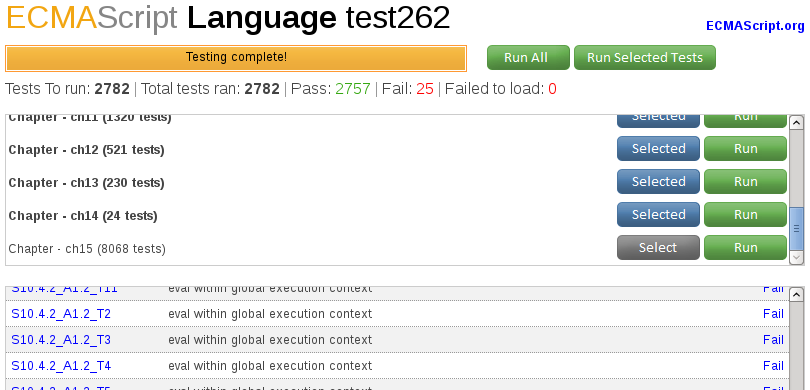
\includegraphics[width = 4cm]{images/test262_small.png}} ;
    \node [below = 0pt of tests] {Test suites} ;

    % \draw<2-> [->, thick] (tests) to node (testing) {} (interp) ;

    % \node<3> [locnode plum, left of = testing] (bisect) {\textsc{Bisect}} ;

    % \draw<3> [->, thick, DarkPlum] (bisect) -- (testing) ;

    % \draw<2-> [<->, thick] (ocaml) -- (jsref) ;

    \draw [<->, thick, Plum] (tests) --
        node [sloped, above, fill = white] {Running tests}
        (jsref) ;

    \node<1> [above of = semlim, locnode brown] (jscert) {JSCert} ;
    \node<2> [dashed, above of = semlim, locnode brown] (jscert) {JSCert} ;

    \draw<1> [->, thick, DarkPlum] (jsref) -- node [above] {Correctness} (jscert) ;
    \draw<2> [->, dashed, thick, DarkPlum] (jsref) -- node [above] {Correctness} (jscert) ;

%   \node [above of = jscert, node distance = 1cm] (next) {} ;
%   \draw [dashed, ->] (jscert) -- (next) ;
%   \node [above of = jscert, left = 3mm, node distance = 1cm] (nextl) {} ;
%   \draw [dashed, ->] (jscert) -- (nextl) ;
%   \node [above of = jscert, right = 3mm, node distance = 1cm] (nextr) {} ;
%   \draw [dashed, ->] (jscert) -- (nextr) ;

    \node [locnode orange, below of = semlim, node distance = 32mm] (ecma) {
\includegraphics[width = 15mm]{images/ecmastandard.png}} ;

    \draw<1> [<->, thick, Plum] (ecma) --
        node [sloped, above, fill = white] {Step / rule}
        node [sloped, below, fill = white] {correspondence} (jscert) ;
    \draw<2> [<->, dashed, thick, Plum] (ecma) --
        node [sloped, above, fill = white] {Step / rule}
        node [sloped, below, fill = white] {correspondence} (jscert) ;

    \draw<2> [<->, thick, Plum] (ecma) --
        node [sloped, below, fill = white] {Step correspondence} (jsref) ;

%    \node [right of = ecma, below, node distance = 3cm] {\texttt{jscert.org}} ;

\end{centertikz}

\end{frame}

\begin{frame}
    \frametitle{Going back to R}

    \begin{block}{R Trust Sources}
        \begin{changemargin}{0pt}{1cm}
    \begin{itemize}
        \item Specification \hfill \xmark
        \item Reference interpreter \hfill \cmark
           \begin{itemize}
               % \item Related by code similarity.
               \item GNU~R.
           \end{itemize}
        \item Test suites \hfill \cmark
           \begin{itemize}
               %\item Related by testing and comparing the results with the reference interpreter.
               \item GNU~R's, FastR's, etc.
           \end{itemize}
        % \item Books and tutoriels (= programmers’s intuition) \hfill \cmark
    \end{itemize}
        \end{changemargin}
    \end{block}

    \begin{block}{Our contributions}
        \begin{itemize}
            \item A Coq interpreter
                \begin{itemize}
                    \item Visually close to the source code of GNU~R;
                    \item Runnable;
                \end{itemize}
            \item A testing architecture.
        \end{itemize}
    \end{block}

\end{frame}

\section{Eyeball closeness}

\sectionframe**{How close CoqR is\\from GNU~R?}{
    \vfill
    \centering{}
    \textcolor{DarkPlum}{Thanks to monads and Coq notations, pretty close.}
}

\begin{frame}[fragile]
    \frametitle{Eyeball Closeness: C Code from GNU~R}

\begin{changemargin}{-5mm}{-5mm}
\begin{ccode}
SEXP do_attr
    (SEXP call, SEXP op, SEXP args, SEXP env){
  SEXP argList, car, ans;
  int nargs = R_length (args);
  argList =
    matchArgs (do_attr_formals, args, call);
  PROTECT (argList);
  if (nargs < 2 || nargs > 3)
    error ("Wrong argument count.");
  car = CAR (argList);
  /* ... */
  return ans;
}
\end{ccode}
\end{changemargin}

\end{frame}

\begin{frame}[fragile]
    \frametitle{Eyeball Closeness: Coq Code from CoqR}

\begin{changemargin}{-5mm}{-5mm}
\begin{coqcode}
Definition do_attr globals runs S
    (call op args env : SEXP) : result SEXP :=
  let%success nargs :=
    R_length globals runs S args using S in
  let%success argList :=
    matchArgs globals runs S
      do_attr_formals args call using S in
  if nargs <? 2 || nargs >? 3 then
    result_error S "Wrong argument count."
  else
    read%list car, _, _ := argList using S in
    (* ... *)
    result_success S ans.
\end{coqcode}
\end{changemargin}

\end{frame}

\begin{frame}[fragile]
    \frametitle{Eyeball Closeness}

    \begin{widemargin}\centering{}
\begin{minipage}{.53\textwidth}
\begin{ccode}[fontsize=\tiny]
SEXP do_attr@\anchorm{nameA}{}@
    (SEXP call, SEXP op, SEXP args, SEXP env){@\anchorm{argsA}{}@
  SEXP argList, car, ans;
  int nargs = R_length (args);@\anchorm{RlengthA}{}@
  argList =@\anchorm{argListA}{}@
    matchArgs (do_attr_formals, args, call);@\anchorm{matchArgsA}{}@
  PROTECT (argList);
  if (nargs < 2 || nargs > 3)@\anchorm{ifA}{}@
    error ("Wrong argument count.");@\anchorm{errorA}{}@
  car = CAR (argList);@\anchorm{carA}{}@
  /* ... */
  return ans;@\anchorm{ansA}{}@
}
\end{ccode}
\end{minipage}
\qquad
\begin{minipage}{.5\textwidth}
\begin{coqcode}[fontsize=\tiny]
@\anchorm{nameB}{}@Definition do_attr globals runs S
    @\anchorm{argsB}{}@(call op args env : SEXP) :=
  let%success nargs :=
    @\anchorm{RlengthB}{}@R_length globals runs S args using S in
  @\anchorm{argListB}{}@let%success argList :=
    @\anchorm{matchArgsB}{}@matchArgs globals runs S
      do_attr_formals args call using S in
  @\anchorm{ifB}{}@if nargs <? 2 || nargs >? 3 then
    @\anchorm{errorB}{}@result_error S "Wrong argument count."
  else
    @\anchorm{carB}{}@read%list car, _, _ := argList using S in
    (* ... *)
    @\anchorm{ansB}{}@result_success S ans.
\end{coqcode}
\end{minipage}
    \end{widemargin}

    \begin{tikzpicture}[overlay, remember picture]
        \def\localxshift{2.5mm} % WTF Tikz…
        \def\localyshift{18mm}
        \draw<2-> [DarkChocolate, thick, <->] ([xshift = \localxshift, yshift = \localyshift]nameA.east) -- ([xshift = \localxshift, yshift = \localyshift]nameB.west) ;
        \draw<2-> [DarkChocolate, thick, <->] ([xshift = \localxshift, yshift = \localyshift]argsA.east) -- ([xshift = \localxshift, yshift = \localyshift]argsB.west) ;
        \draw<2-> [DarkChocolate, thick, <->] ([xshift = \localxshift, yshift = \localyshift]RlengthA.east) -- ([xshift = \localxshift, yshift = \localyshift]RlengthB.west) ;
        \draw<2-> [DarkChocolate, thick, <->] ([xshift = \localxshift, yshift = \localyshift]argListA.east) -- ([xshift = \localxshift, yshift = \localyshift]argListB.west) ;
        \draw<2-> [DarkChocolate, thick, <->] ([xshift = \localxshift, yshift = \localyshift]matchArgsA.east) -- ([xshift = \localxshift, yshift = \localyshift]matchArgsB.west) ;
        \draw<2-> [DarkChocolate, thick, <->] ([xshift = \localxshift, yshift = \localyshift]ifA.east) -- ([xshift = \localxshift, yshift = \localyshift]ifB.west) ;
        \draw<2-> [DarkChocolate, thick, <->] ([xshift = \localxshift, yshift = \localyshift]errorA.east) -- ([xshift = \localxshift, yshift = \localyshift]errorB.west) ;
        \draw<2-> [DarkChocolate, thick, <->] ([xshift = \localxshift, yshift = \localyshift]carA.east) -- ([xshift = \localxshift, yshift = \localyshift]carB.west) ;
        \draw<2-> [DarkChocolate, thick, <->] ([xshift = \localxshift, yshift = \localyshift]ansA.east) -- ([xshift = \localxshift, yshift = \localyshift]ansB.west) ;
    \end{tikzpicture}

    \begin{block}<3>{Not an exact match, but easily verifiable}
        \begin{itemize}
            \item Monads encode the semantics of GNU~R;
            \item Coq notations ease the line-to-line correspondence;
            \item Main differences:
                \begin{itemize}
                    \item the global state is propagated all along;
                    \item no garbage collection.
                \end{itemize}
        \end{itemize}
    \end{block}

\end{frame}

\section{Testing Framework}

\begin{frame}

    \begin{centertikz}

        \node [box] (coqR) {CoqR (Coq)} ;

        % \onslide<3->{
        %     \node [box, left = 5mm of coqR] (Rlibraries) {\parbox{5em}{\centering{}R base\\library (R)}} ;
        %     \draw [->, DarkPlum, thick] (Rlibraries) to [bend left = 50] (coqR) ;
        %     \draw [->, DarkSkyBlue, thick] (Rlibraries) to [bend right = 50]
        %         node [below, DarkSkyBlue] {Initial state} (coqR) ;
        % }

        \node [box, right = 3cm of coqR] (gnuR) {GNU~R (C)} ;

        \draw [<->, DarkChocolate, thick] (coqR) --
            node [above, DarkChocolate] (llc) {line-by-line}
            node [below, DarkChocolate] {correspondence} (gnuR) ;

        \onslide<2->{
            \node [box, above = 2cm of llc] (tests) {test suites (R)} ;
            \draw [->, DarkPlum, thick] (tests) to [out = -90, in = 90] (coqR) ;
            \draw [->, DarkPlum, thick] (tests) to [out = -90, in = 90] node [right, near end, xshift = 1mm] {execute} (gnuR) ;
        }

        \onslide<3->{
            \node [right = 1cm of tests] (testinstances) {%
                \hspace{-1em}%
                \begin{minipage}{25mm}
                \begin{itemize}
                    \item GNU~R's;
                    \item FastR's;
                    \item Corners.
                \end{itemize}
                \end{minipage}%
            } ;
            \draw [->, Aluminium6] (tests) -- (testinstances);
            \draw [decorate, decoration = {brace, amplitude = 10pt}, DarkPlum] (testinstances.north east) --
               node [xshift = 4mm, right, DarkPlum] {\parbox{4em}{\(20,000\)\\expressions}} (testinstances.south east) ;
        }

        \onslide<2-3>{
            \node [box, below = 2cm of coqR] (resultCoqR) {output} ;
            \node [box, below = 2cm of gnuR] (resultGnuR) {output} ;
            \draw [->, DarkSkyBlue, thick] (coqR) -- (resultCoqR) ;
            \draw [->, DarkSkyBlue, thick] (gnuR) -- node [right] {results} (resultGnuR) ;
            \draw [<->, DarkScarletRed, thick] (resultCoqR) --
               node [above] {compare} (resultGnuR) ;
        }

        \onslide<4->{
            \newcommand\identifytype{\parbox{5.5em}{\centering{}Identify type\\of results}}
            \node [box, below = 15mm of coqR] (typeCoqR) {\identifytype} ;
            \node [box, below = 15mm of gnuR] (typeGnuR) {\identifytype} ;
            \draw [->, DarkSkyBlue, thick] (coqR) -- (typeCoqR) ;
            \draw [->, DarkSkyBlue, thick] (gnuR) -- node [right] {results} (typeGnuR) ;
            \draw [<->, DarkScarletRed, thick] (typeCoqR) --
               node [above] {compare types} (typeGnuR) ;
            \newcommand\interpretetresult{\parbox{3.5em}{\centering{}Interpret\\results}}
            \node [box, below = 1cm of typeCoqR] (interCoqR) {\interpretetresult} ;
            \node [box, below = 1cm of typeGnuR] (interGnuR) {\interpretetresult} ;
            \draw [->, DarkSkyBlue, thick] (typeCoqR) -- (interCoqR) ;
            \draw [->, DarkSkyBlue, thick] (typeGnuR) -- (interGnuR) ;
            \draw [<->, DarkScarletRed, thick] (interCoqR) --
               node [above] {compare} node [below] {interpretations} (interGnuR) ;
        }

        \onslide<5->{
            \node [right = 5mm of typeGnuR] (types) {%
                \hspace{-1em}%
                \begin{minipage}{37mm}
                \begin{itemize}
                    \item Boolean vector;
                    \item Numeric vector;
                    \item …
                    \item Closure;
                    \item Error;
                    \onslide<6->{
                    \item Not implemented;
                    \item Impossible;
                    \item Unknown.
                    }
                \end{itemize}
                \end{minipage}%
            } ;
            \draw [->, Aluminium6] (typeGnuR) -- (types);
        }

    \end{centertikz}

\end{frame}

\begin{frame}
    \begin{center}
        \vspace{-2mm}
        \href{https://coqr.dcc.uchile.cl/\#/test-detail/148}{\url{https://coqr.dcc.uchile.cl}}
        \vspace{2mm}
        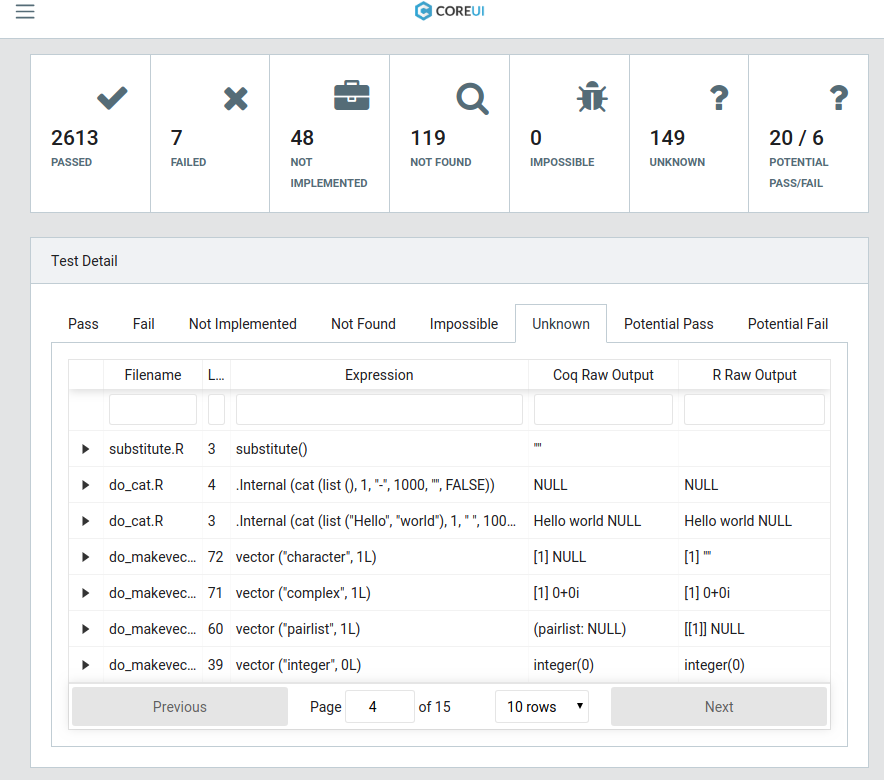
\includegraphics[width=10cm]{images/unknown.png}
    \end{center}
\end{frame}

% \begin{frame}

%     \begin{center}
%         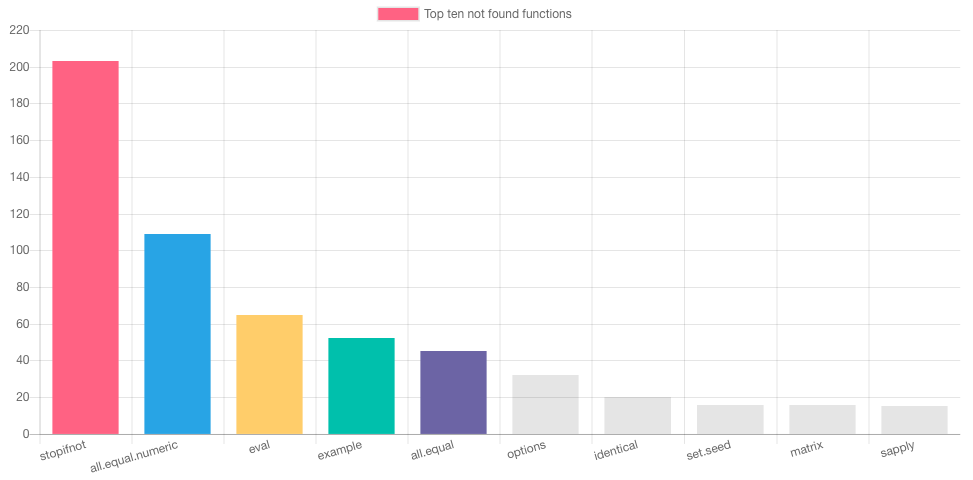
\includegraphics[width=10cm]{../missing_functions_base_r.png}
%     \end{center}

% \end{frame}

\begin{frame}
    \frametitle{Identifying low-hanging fruits}

    \begin{center}
        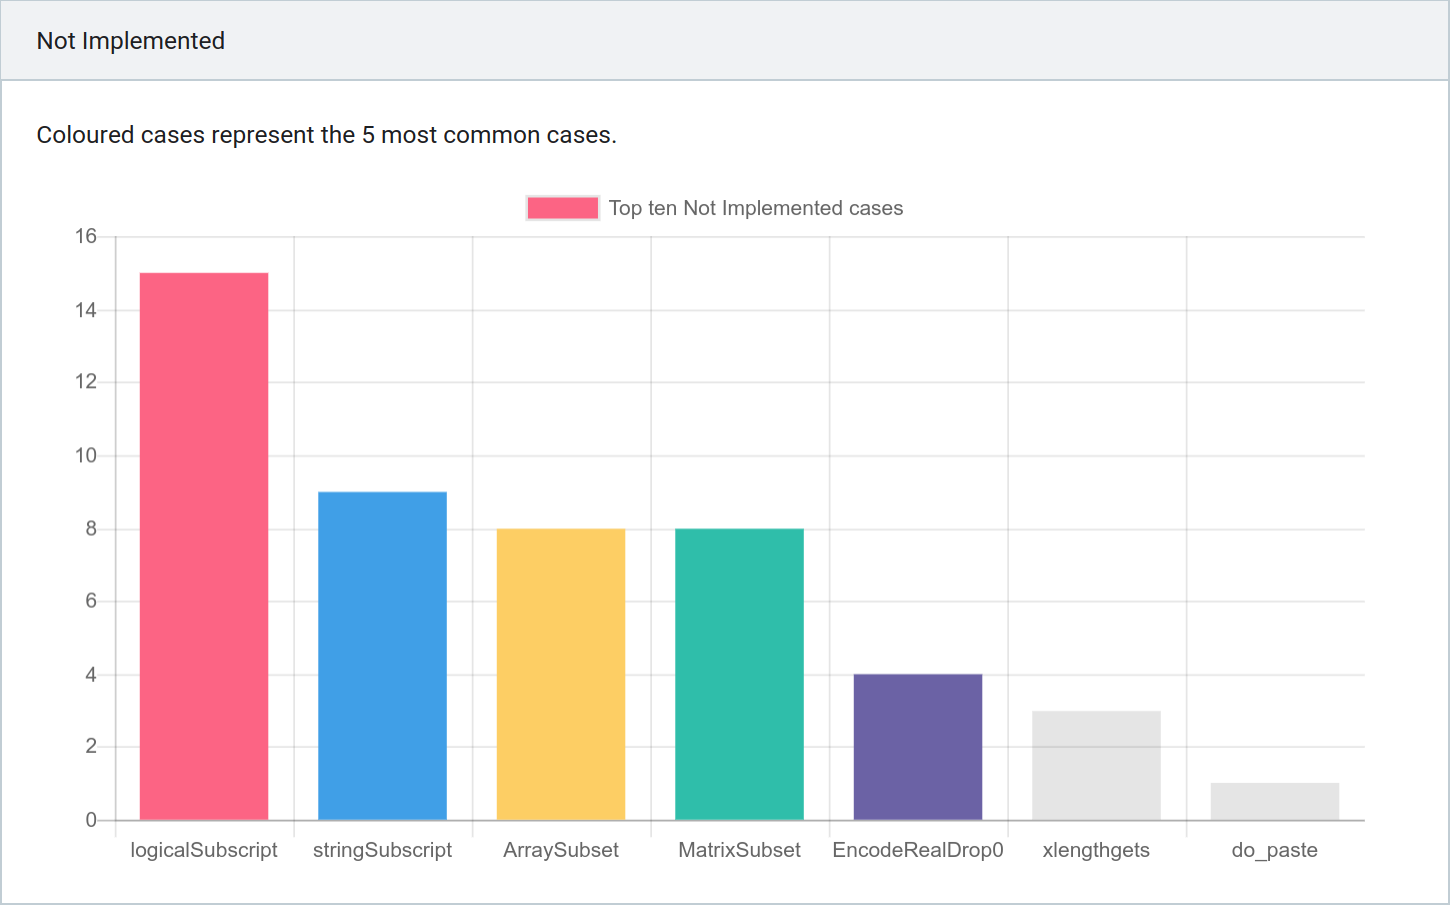
\includegraphics[width=10cm]{images/not-implemented.png}
    \end{center}

    \pause
    CoqR supports a \emphb{non-trivial} subset of R, and fully support them.

\end{frame}

\begin{frame}
    \frametitle{This way of doing things is generic!}

    From:
    \begin{itemize}
        \item Two interpreters with similar inputs;
        \item A set of result types;
        \item A meaningful way to interpreter these results
    \end{itemize}
    We get:
    \begin{itemize}
        \item A customized testing framework;
        \item Meaningful testing results;
        \item A way to prioritise functions to be implemented.
    \end{itemize}

    \pause
    \vfill
    \begin{block}{Bonus}
        The eyeball closeness made debugging trivial.
    \end{block}

\end{frame}

\begin{frame}
    \only<1>{\frametitle{Conclusion}}
    \only<2>{\frametitle{Thank you for listening!}}

    \begin{centertikz}

        \node [box] (coqR) {CoqR (Coq)} ;

        % \onslide<3->{
        %     \node [box, left = 5mm of coqR] (Rlibraries) {\parbox{5em}{\centering{}R base\\library (R)}} ;
        %     \draw [->, DarkPlum, thick] (Rlibraries) to [bend left = 50] (coqR) ;
        %     \draw [->, DarkSkyBlue, thick] (Rlibraries) to [bend right = 50]
        %         node [below, DarkSkyBlue] {Initial state} (coqR) ;
        % }

        \node [box, right = 3cm of coqR] (gnuR) {GNU~R (C)} ;

        \draw [<->, DarkChocolate, thick] (coqR) --
            node [above, DarkChocolate] (llc) {line-by-line}
            node [below, DarkChocolate] {correspondence} (gnuR) ;

            \node [box, above = 11mm of llc] (tests) {test suites (R)} ;
            \draw [->, DarkPlum, thick] (tests) to [out = -90, in = 90] (coqR) ;
            \draw [->, DarkPlum, thick] (tests) to [out = -90, in = 90] node [right, near end, xshift = 1mm] {execute} (gnuR) ;

            \newcommand\identifytype{\parbox{5.5em}{\centering{}Identify type\\of results}}
            \node [box, below = 9mm of coqR] (typeCoqR) {\identifytype} ;
            \node [box, below = 9mm of gnuR] (typeGnuR) {\identifytype} ;
            \draw [->, DarkSkyBlue, thick] (coqR) -- (typeCoqR) ;
            \draw [->, DarkSkyBlue, thick] (gnuR) -- node [right] {results} (typeGnuR) ;
            \draw [<->, DarkScarletRed, thick] (typeCoqR) --
               node [above] {compare types} (typeGnuR) ;
            \newcommand\interpretetresult{\parbox{3.5em}{\centering{}Interpret\\results}}
            \node [box, below = 5mm of typeCoqR] (interCoqR) {\interpretetresult} ;
            \node [box, below = 5mm of typeGnuR] (interGnuR) {\interpretetresult} ;
            \draw [->, DarkSkyBlue, thick] (typeCoqR) -- (interCoqR) ;
            \draw [->, DarkSkyBlue, thick] (typeGnuR) -- (interGnuR) ;
            \draw [<->, DarkScarletRed, thick] (interCoqR) --
               node [above] {compare} node [below] {interpretations} (interGnuR) ;

    \end{centertikz}

    \begin{center}
        \url{https://github.com/Mbodin/CoqR}
        \href{https://coqr.dcc.uchile.cl/\#/test-detail/148}{\url{https://coqr.dcc.uchile.cl}}
    \end{center}

\end{frame}

\frame{\tableofcontents}

\sectionframe*{Bonuses}

\newcommand\questiontoc{
    %\begin{multicols}{2}
    \begin{enumerate}
        \item \hyperlink{frame:Rlazy}{R: A Lazy Programming Language};
        \item \hyperlink{frame:jscert}{JSCert{}};
        \item \hyperlink{frame:imperative:functional}{Representing imperativity in a functional setting};
        \item \hyperlink{frame:semantics:coq}{Semantics in Coq};
        \item \hyperlink{frame:semantic:sizes}{Semantic sizes};
        \item \hyperlink{frame:other:subtleties}{Other Subtleties of R};
        \item \hyperlink{frame:reading:pointers}{Reading pointers};
        \item \hyperlink{frame:parser}{Parsing R};
        \item \hyperlink{frame:eyeball}{The eyeball closeness};
        \item \hyperlink{frame:full:monad}{The full monad};
        \item \hyperlink{frame:RFeatures}{R features};
        \item \hyperlink{frame:input:output}{Inputs and outputs};
        \item \hyperlink{frame:proofs}{Proofs};
        \item \hyperlink{frame:proofs:future}{Future of proofs};
        \item \hyperlink{frame:ble}{Basic language elements in memory};
        \item \hyperlink{frame:fails}{More details about the website’s results};
        \item \hyperlink{frame:full:results}{Full testing results}.
    \end{enumerate}
    %\end{multicols}
}

\frame{\questiontoc}

\begin{frame}[fragile]
    \label{frame:Rlazy}
    \frametitle{R: A Lazy Programming Language}

\begin{Rcode}
f <- function (x, y = x) {
    x <- 1
    y
    x <- 2
    y
}
f (3)                               @\pause@# Returns 1
\end{Rcode}

\begin{overlayarea}{\textwidth}{3cm}
\begin{onlyenv}<3->
\begin{Rcode}
f <- function (x, y) if (x == 1) y
f (1, a <- 1)
a                                   # Returns 1
f (0, b <- 1)
b                                   # Raises an error
\end{Rcode}
\end{onlyenv}
\end{overlayarea}

\end{frame}

\frame{\questiontoc}

\begin{frame}
    \label{frame:jscert}
    \frametitle{The JSCert{} Project
        \hfill\hfill\hfill
        \raisebox{-10mm}[0pt][0pt]{
            
\includegraphics[width = 15mm]{images/jscert.png} ;
        }}

\begin{centertikz}[node distance = 1.5cm]

    \node (realworldleft) {};
    \node [right of = realworldleft, node distance = 11.5cm] (realworldright) {} ;

    \node [right of = realworldleft, node distance = 1.5cm] (semlim) {} ;
    \node [left of = realworldright, node distance = 4cm] (testlim) {} ;

    \draw [dashed] (realworldleft) to node[above, pos = 0.9] {Coq definitions} node [below, pos = 0.9] {Industrial world} (realworldright) ;

    % \node<2-> [below of = testlim, locnode] (ocaml) {\parbox{1.5cm}{\centering\camln{}\\extraction}} ;
    % \node<2-> [right of = ocaml, node distance = 2cm, locnode] (parser) {Parser} ;

\begin{pgfonlayer}{background}
    % \node<2-> [fit = (ocaml) (parser), locnode yellow] (interp) {} ;
\end{pgfonlayer}

    \node [above of = testlim, locnode brown] (jsref) {JSRef} ;
    \node [above = 0pt of jsref] {\(\sim{}3,000\)~lines of code} ;

    \node [locnode blue, below of = jsref, node distance = 45mm] (tests) {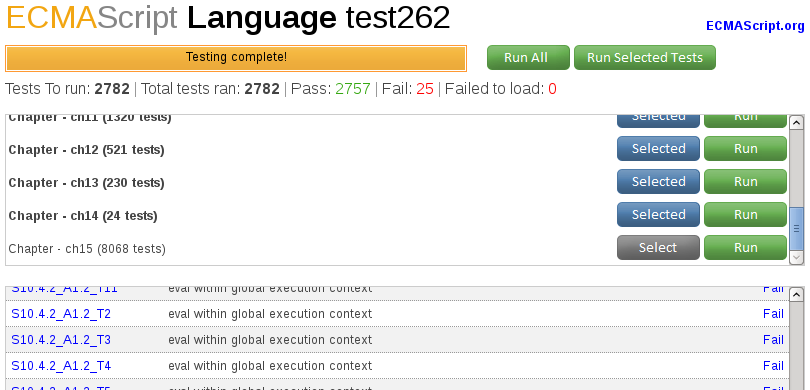
\includegraphics[width = 4cm]{images/test262_small.png}} ;
    \node [below = 0pt of tests] {\(5,126\)~tests passed} ; % out of~\(11,725\)} ;

    % \draw<2-> [->, thick] (tests) to node (testing) {} (interp) ;

    % \node<3> [locnode plum, left of = testing] (bisect) {\textsc{Bisect}} ;

    % \draw<3> [->, thick, DarkPlum] (bisect) -- (testing) ;

    % \draw<2-> [<->, thick] (ocaml) -- (jsref) ;

    \draw [<->, thick, Plum] (tests) --
        node [sloped, above, fill = white] {Running tests}
        (jsref) ;

    \node [above of = semlim, locnode brown] (jscert) {JSCert} ;
    \node [above = 0pt of jscert] {\(\sim{}900\)~rules} ;

    \draw [->, thick, DarkPlum] (jsref) -- node [above] {Correctness}
            node [below, Aluminium6] {\(\sim{}6,000\)~lines of proof} (jscert) ;

%   \node [above of = jscert, node distance = 1cm] (next) {} ;
%   \draw [dashed, ->] (jscert) -- (next) ;
%   \node [above of = jscert, left = 3mm, node distance = 1cm] (nextl) {} ;
%   \draw [dashed, ->] (jscert) -- (nextl) ;
%   \node [above of = jscert, right = 3mm, node distance = 1cm] (nextr) {} ;
%   \draw [dashed, ->] (jscert) -- (nextr) ;

    \node [locnode orange, below of = semlim, node distance = 32mm] (ecma) {
\includegraphics[width = 15mm]{images/ecmastandard.png}} ;
    \node [below = 0pt of ecma] {\(\sim{}900\)~steps} ;

    \draw [<->, thick, Plum] (ecma) --
        node [sloped, above, fill = white] {Step / rule}
        node [sloped, below, fill = white] {correspondence} (jscert) ;


%    \node [right of = ecma, below, node distance = 3cm] {\texttt{jscert.org}} ;

\end{centertikz}

\end{frame}

\frame{\questiontoc}

\begin{frame}[fragile]
    \label{frame:imperative:functional}
    \frametitle{How to Represent Imperative Features in a Functional Setting}

    \begin{itemize}
        \item Structures like maps are easy to implement;
        \item We can represent every element of the state of a program \\
            (memory, outputs, etc.) in a data-structure;
        \item We have to pass this structure along the program.
    \end{itemize}

    \begin{block}{Enter the monad}
\begin{camlcode}
if_success (run s1 p) (fun s2 =>
  let s3 = write s2 x v in
  if_success (run s3 p') (fun s4 =>
    return_success s4))
\end{camlcode}
    \end{block}

\end{frame}

\frame{\questiontoc}

\begin{frame}[fragile]
    \label{frame:semantics:coq}
    \frametitle{Formalisation of Semantics in Coq}

\begin{coqcode}
Inductive semantics : state -> prog -> state -> Prop ->

  | semantics_skip : forall s p, semantics s p s

  | semantics_seq : forall s1 s2 s3 p1 p2,
    semantics s1 p1 s2 ->
    semantics s2 p2 s3 ->
    semantics s1 (seq p1 p2) s3

  | semantics_asgn : forall s x v,
    semantics s (asgn x v) (write s x v)
  .
\end{coqcode}

\end{frame}

\begin{frame}
    \frametitle{Sequence in JSCert{} (Paper Version)}

    \begin{overlayarea}{\textwidth}{3cm}
    \begin{block}{“\jsinline|s1 ; s2|” is evaluated as follows.}
\begin{enumerate}
    \item Let~\(o_1\) be the result of evaluating~\jsinline|s1|.
    \item If~\(o_1\) is an exception, return~\(o_1\).
    \item Let~\(o_2\) be the result of evaluating~\jsinline|s2|.
    \only<1>{
        \item If an exception~\(\mathit{V}\) was thrown, return \(\mpar{\mathtt{throw}, \mathit{V}, \mathit{empty}}\). % where \(\mathit{V}\)~is the exception.
            % (Execution now proceeds as if no exception were thrown.)
        \item If~\(\mathit{o_2}.\mathit{value}\) is empty, let~\(\mathit{V} = \mathit{o_1}.\mathit{value}\),
            otherwise let~\(\mathit{V} = \mathit{o_2}.\mathit{value}\).
        \item Return \(\mpar{\mathit{o_2}.\mathit{type}, \mathit{V}, \mathit{o_2}.\mathit{target}}\).
    }
\end{enumerate}
    \end{block}
    \end{overlayarea}

    \visible<3>{
\begin{mathpar}
    \inferrule[seq-1\(\fund{s_1}{s_2}\)]
    { S, C, s_1 \evalr o_1 \\ o_1, \seqx{s_2} \evalr o }
    { S, C, \seq{s_1}{s_2} \evalr o }
    \and
    \inferrule[seq-2\(\funu{s_2}\)]
    { }
    { o_1, \seqx{s_2} \evalr o_1 }
    \quad { \abort{o_1} }
    \and
    \inferrule[seq-3\(\funu{s_2}\)]
    { o_1, s_2 \evalr o_2 \\ o_1, o_2, \seqxx{} \evalr o }
    { o_1, \seqx{s_2} \evalr o }
    \quad { \neg\abort{o_1} }
    \and
    \ldots
\end{mathpar}
}

\end{frame}

\begin{frame}[fragile]
    \label{frame:seq:jscert}
    \frametitle{Sequence in JSCert{}}

%  | red_stat_abort : forall S C extt o,
%    out_of_ext_stat extt = Some o ->
%    abort o ->
%    ~ abort_intercepted_stat extt ->
%    red_stat S C extt o

\begin{changemargin}{-5.5mm}{-9mm}
\begin{coqcode}
Inductive red_stat : state -> scope -> stat -> out -> Prop :=

| red_stat_seq_1 : forall S C s1 s2 o1 o,
  red_stat S C s1 o1 ->
  red_stat S C (seq_1 s2 o1) o ->@\anchor{seq1}{}@
  red_stat S C (seq s1 s2) o

| red_stat_seq_2 : forall S C s2 o1,
  abort o1 ->@\anchor{seq2}{}@
  red_stat S C (seq_1 s2 o1) o1

| red_stat_seq_3 : forall S0 S C s2 o2 o,
  red_stat S C s2 o2 ->@\anchor{seq3}{}@
  red_stat S C (seq_2 o2) o ->
  red_stat S0 C (seq_1 s2 (out_ter S)) o

(* ... *).
\end{coqcode}
\end{changemargin}
\onslide<2>{%
\begin{innertikz}[overlay, remember picture]
    \def\distshift{35mm} % WTF: This looks like a TikZ bug: nodes appear this distance below their supposed location…
    \node [right = 15mm of seq1, yshift = \distshift, scale = .8] {\(
        \inferrule[seq-\raisebox{.6ex}{\bsphere{1}}\(\fund{s_1}{s_2}\)]
        { S, C, s_1 \evalr o_1 \\ o_1, \seqx{s_2} \evalr o }
        { S, C, \seq{s_1}{s_2} \evalr o }
    \)} ;
    \node [right = 61mm of seq2, yshift = \distshift, scale = .8] {\(
        \inferrule[seq-\raisebox{.6ex}{\bsphere{2}}\(\funu{s_2}\)]
        { }
        { o_1, \seqx{s_2} \evalr o_1 }
        \quad { \abort{o_1} }
    \)} ;
    \node [right = 28mm of seq3, yshift = \distshift, scale = .7] {\(
        \inferrule[seq-\raisebox{.55ex}{\bsphere{3}}\(\funu{s_2}\)]
        { o_1, s_2 \evalr o_2 \\ o_1, o_2, \seqxx{} \evalr o }
        { o_1, \seqx{s_2} \evalr o }
        \quad { \neg\abort{o_1} }
    \)} ;
\end{innertikz}}

\end{frame}

\frame{\questiontoc}

\begin{frame}
    \label{frame:semantic:sizes}
    \frametitle{Semantic Sizes}

    \vspace{-5mm}

    \begin{centertikz}[scale=.5]

        \node (lambda) {\(\lambda\)-calculus} ;
        \node [right = 5mm of lambda] (ml) {CoreML} ;
        \node [right = 5mm of ml] (compcert) {CompCert{} C} ;
        \node [right = 5mm of compcert] (jscert) {JSCert{}} ;
        \node [right = 5mm of jscert] (coqR) {CoqR{}} ;

        \draw [DarkPlum, fill = LightPlum] ($(lambda.north) + (-.5, .1)$) rectangle ++ (1, .003) ;
        \node [above = 1mm of lambda] {\(3\)~rules} ; % 5 in pretty-big-step.

        \draw [DarkPlum, fill = LightPlum] ($(ml.north) + (-.5, .1)$) rectangle ++ (1, .25) ;
        \node [above = 2mm of ml] {\(\sim{}50\)~rules} ; % 61 in pretty-big-step.

        \draw [DarkPlum, fill = LightPlum] ($(compcert.north) + (-.5, .1)$) rectangle ++ (1, 1) ;
        \node [above = 6mm of compcert] {\(\sim{}200\)~rules} ; % 110 in big step + 77 in denotational.
        % Source: http://compcert.inria.fr/doc/html/Csem.html and http://compcert.inria.fr/doc/html/Cop.html

        \draw [DarkPlum, fill = LightPlum] ($(jscert.north) + (-.5, .1)$) rectangle ++ (1, 4.5) ;
        \node [above = 23mm of jscert] {\(\sim{}900\)~rules} ; % ~900 in pretty-big-step.

        \draw [DarkPlum, fill = LightPlum] ($(coqR.north) + (-.5, .1)$) rectangle ++ (1, 10) ;
        \node [above = 50mm of coqR] {\(\sim{}2,000\)~rules} ; % 2028 occurrences of 'let%'.

%        \draw [thick, dashed, ->] (compcert) to [bend right] ($(compcert) + (-1, -1)$) ;

    \end{centertikz}
%    \vspace{-5mm}

%   \begin{refsection}
%       \nocite{Verasco}
%       \printbibliography{}
%   \end{refsection}

    \begin{block}{}
    (Estimation of the size of each project if we were to entirely translate them into a small-step semantics.)
    \end{block}

    ~\vfill

    ~\vfill

\end{frame}

\frame{\questiontoc}

\begin{frame}[fragile]
    \label{frame:other:subtleties}
    \frametitle{Other Subtleties}

%\begin{onlyenv}<1>
\begin{Rcode}
f <- function (x, y, option, longArgumentName) ...

# All the following calls are equivalent.
f (1, 2, "something", 42)
f (option = "something", 1, 2, 42)
f (opt = "something", long = 42, 1, 2)
\end{Rcode}
%\end{onlyenv}

\begin{overlayarea}{\textwidth}{5cm}
\begin{onlyenv}<2>
\begin{Rcode}
f <- function (abc, ab, de) c (abc, ab, de)

# All the following calls are equivalent.
f (1, 2, 3)
f (de = 3, 1, 2)
f (d = 3, 1, 2)
f (ab = 2, 1, 2)
f (ab = 2, a = 1, 3)

f (a = 3, 1, 2) # Returns an error.
\end{Rcode}
\end{onlyenv}
\end{overlayarea}

\end{frame}

\frame{\questiontoc}

\begin{frame}[fragile]
    \label{frame:reading:pointers}
    \frametitle{Eyeball Closeness: Reading Pointers}

    \begin{changemargin}{-5mm}{-5mm}

\begin{minipage}{.6\textwidth}
    {C code}
\begin{ccode}
symsxp_struct p_sym = p->symsxp;
/* ... */
\end{ccode}
\end{minipage}
    \begin{minipage}{.45\textwidth}
    \begin{itemize}
        \item May fail because the pointer \cinline|p| is unbound;
        \item May fail because the union \cinline|*p| is not a \cinline|symsxp|.
    \end{itemize}
    \end{minipage}

\vfill

\parbox{\textwidth}{\onslide<2->{Coq code, \only<2>{first}\only<3>{second}\only<4>{third}\only<5>{fourth} try}}
\begin{minipage}{.5\textwidth}
\begin{overlayarea}{\textwidth}{5cm}
    \begin{onlyenv}<2>
\begin{coqcode}
match read p with
  (* ... *)
end
\end{coqcode}
    \end{onlyenv}
    \begin{onlyenv}<3>
\begin{coqcode}
match read S p with
| Some p_ =>
  match p_ with
  | symSxp p_sym =>
    (* ... *)
  | _ => (* ??? *)
  end
| None => (* ??? *)
end
\end{coqcode}
    \end{onlyenv}
    \begin{onlyenv}<4>
\begin{coqcode}
match read S p with
| Some p_ =>
  match p_ with
  | symSxp p_sym =>
    (* ... *)
  | _ => error
  end
| None => error
end
\end{coqcode}
    \end{onlyenv}
    \begin{onlyenv}<5>
\begin{coqcode}
read%sym p_sym :=
  p using S in
(* ... *)
\end{coqcode}
    \end{onlyenv}
\end{overlayarea}
\end{minipage}\quad
\begin{minipage}{.5\textwidth}
\begin{minipage}{1.2\textwidth}
\begin{overlayarea}{\textwidth}{5cm}
    \begin{onlyenv}<4->
\begin{coqcode}
Inductive result (T : Type) :=
  | success : state -> T
              -> result T
  | error : result T
  .
\end{coqcode}
    \end{onlyenv}
    \begin{onlyenv}<5->
\begin{coqcode}
Notation "'read%sym' p_sym ':='
    p 'using' S 'in' cont" :=
  (* ... *).
\end{coqcode}
    \end{onlyenv}
\end{overlayarea}
\end{minipage}
\end{minipage}

\end{changemargin}

\end{frame}

\frame{\questiontoc}

\begin{frame}[fragile]
    \label{frame:parser}

\begin{textcodenoescape}
expr:
  | NUM_CONST              { $$ = $1;  setId( $$, @$); }
  | STR_CONST              { $$ = $1;  setId( $$, @$); }
  | NULL_CONST             { $$ = $1;  setId( $$, @$); }          
  | SYMBOL                 { $$ = $1;  setId( $$, @$); }
  | LBRACE exprlist RBRACE
    { $$ = xxexprlist($1,&@1,$2); setId( $$, @$); }
  | LPAR expr_or_assign RPAR
    { $$ = xxparen($1,$2);  setId( $$, @$); }
\end{textcodenoescape}

\begin{camlcode}
expr:
  | c = NUM_CONST                       { c }
  | c = STR_CONST                       { c }
  | c = NULL_CONST                      { c }
  | c = SYMBOL                          { c }
  | b = LBRACE; e = exprlist; RBRACE
    { eatLines := false ;
      lift2 (only_state xxexprlist) b e }
  | p = LPAR; e = expr_or_assign; RPAR
    { lift2 (no_runs xxparen) p e }
\end{camlcode}

\end{frame}

\frame{\questiontoc}

\sectionframe**{Eyeball Closeness}{
    \label{frame:eyeball}
    \begin{itemize}
        \item C is imperative, pointer-based;
        \item Coq is purely functional, value-based;
        \item The translation is based on a monad \(\mathrm{state}+\mathrm{error}\).
    \end{itemize}
}

\begin{frame}[fragile]
    \frametitle{Eyeball Closeness: Enumeration}

    \begin{minipage}{.45\textwidth}
        C code

\begin{ccode}
typedef enum {
    NILSXP  = 0,
    SYMSXP  = 1,
    LISTSXP = 2,
    CLOSXP  = 3,
    ENVSXP  = 4,
    PROMSXP = 5,
    /* ... */
} SEXPTYPE;
\end{ccode}

    \end{minipage}
    \qquad
    \begin{minipage}{.45\textwidth}
        Coq code

\begin{coqcode}
Inductive SExpType :=
  | NilSxp
  | SymSxp
  | ListSxp
  | CloSxp
  | EnvSxp
  | PromSxp
  (* ... *)
  .
\end{coqcode}

    \end{minipage}

    %\begin{itemize}
    %    \item Enumerations are actually more natural in Coq than in C.
    %\end{itemize}

\end{frame}

\begin{frame}[fragile]
    \frametitle{Eyeball Closeness: Records}

        \begin{widemargin}
            \centering{}
    \begin{minipage}{.5\textwidth}
        C code

\begin{ccode}
struct sxpinfo_struct {
  SEXPTYPE type      :  5;
  unsigned int obj   :  1;
  unsigned int named :  2;
  unsigned int gp    : 16;
  unsigned int mark  :  1;
  unsigned int debug :  1;
  unsigned int trace :  1;
  unsigned int spare :  1;
  unsigned int gcgen :  1;
  unsigned int gccls :  3;
};
/* Total: 32 bits */
\end{ccode}

    \end{minipage}
    \qquad
    \begin{minipage}{.47\textwidth}
        Coq code

\begin{coqcode}
Inductive named_field :=
  | named_temporary
  | named_unique
  | named_plural
  .

Record SxpInfo :=
  make_SxpInfo {
    type : SExpType ;
    obj : bool ;
    named : named_field ;
    gp : nbits 16
  }.
\end{coqcode}

    \end{minipage}
    \end{widemargin}

    %\begin{itemize}
    %    \item We recognise some formalisation choices,
    %        but still close enough.
    %\end{itemize}

\end{frame}

\begin{frame}[fragile]
    \frametitle{Eyeball Closeness: Unions}

    \begin{changemargin}{-5mm}{-5mm}
\begin{minipage}{.8\textwidth}
\begin{ccode}
union {
    struct primsxp_struct primsxp;
    struct symsxp_struct symsxp;
    struct listsxp_struct listsxp;
    /* ... */
};
\end{ccode}
\end{minipage}
    \begin{minipage}{.18\textwidth}
    \textbf{C code}\\

    Accesses are unsafe.
    \end{minipage}

\begin{minipage}{.8\textwidth}
\begin{coqcode}
Inductive SExpRec_union :=
  | primSxp : PrimSxp_struct -> SExpRec_union
  | symSxp : SymSxp_struct -> SExpRec_union
  | listSxp : ListSxp_struct -> SExpRec_union
  (* ... *)
  .
\end{coqcode}
\end{minipage}
    \begin{minipage}{.18\textwidth}
    \textbf{Coq code}\\

    Accesses must be guarded.
    \end{minipage}
\end{changemargin}

    %\begin{itemize}
    %    \item Large conceptual differences,
    %        but still an eyeball closeness in the definitions.
    %\end{itemize}

\end{frame}

\begin{frame}[fragile]
    \frametitle{Eyeball Closeness: Reading Pointers}

    \vspace{-1mm}
    \begin{changemargin}{-10mm}{-10mm}\centering{}
\begin{minipage}{.57\textwidth}
    {C code}
\begin{ccode}
symsxp_struct p_sym = p->symsxp;
/* ... */
\end{ccode}
\end{minipage}\hspace{6mm}%
\begin{minipage}{.54\textwidth}
    {Coq code}
\begin{coqcode}
read%sym p_sym := p using S in
(* ... *)
\end{coqcode}
\end{minipage}
    \end{changemargin}
    \vspace{-1mm}

\begin{coqcode}
Inductive result (T : Type) :=
  | result_success : state -> T -> result T
  | result_error : result T.
\end{coqcode}

\begin{coqcode}
Notation "'read%sym' p_sym ':=' p 'using' S 'in' cont" :=
  (match read S p with
   | Some p_ =>
     match p_ with
     | symSxp p_sym => cont
     | _ => result_error
     end
   | None => result_error
   end).
\end{coqcode}

\end{frame}

\frame{\questiontoc}

\begin{frame}[fragile]
    \label{frame:full:monad}
    \frametitle{The Full State+Error Monad}

\begin{coqcode}
Inductive result (A : Type) :=
  | result_success : state -> A -> result A
  | result_error : state -> string -> result A
  | result_longjump : state -> nat -> context_type
                      -> result A
  | result_impossible : state -> string -> result A
  | result_not_implemented : string -> result A
  | result_bottom : state -> result A
  .
\end{coqcode}

\end{frame}

\frame{\questiontoc}

\begin{frame}[fragile]
    \label{frame:input:output}

\begin{coqcode}
Record input := make_input {
    prompt_string : stream string ;
    random_boolean : stream bool
  }.
\end{coqcode}

\begin{coqcode}
Record output := make_output {
    output_string : list string
  }.
\end{coqcode}

\begin{coqcode}
Record state := make_state {
    inputs :> input ;
    outputs :> output ;
    state_memory :> memory ;
    state_context : context
  }.
\end{coqcode}

\end{frame}

\frame{\questiontoc}

\sectionframe**{R Features}{\label{frame:RFeatures}}

\begin{frame}[fragile]
    \frametitle{R Core}

\begin{ccode}
FUNTAB R_FunTab[] = {
  {"if",        do_if,        2},
  {"while",     do_while,     2},
  {"break",     do_break,     0},
  {"return",    do_return,    1},
  {"function",  do_function,  -1},
  {"<-",        do_set,       2},
  {"(",         do_paren,     1},
  /* ... */
  {"+",         do_arith1,    2},
  {"-",         do_arith2,    2},
  {"*",         do_arith3,    2},
  {"/",         do_arith4,    2},
  /* ... */
  {"cos",       do_math20,    1},
  {"sin",       do_math21,    1},
  {"tan",       do_math22,    1},
  /* ... */ }
\end{ccode}

    \begin{overlayarea}{\textwidth}{0cm}
        \only<2>{
            \vspace{-8cm}
            \parbox[t]{0pt}{
                \centering{}~\hspace{-1cm}%
                \tikz \fill[white] (0, 0) rectangle (12, 6) ;
            }%
            \vspace{-6cm} % WTF KNUTH
            \begin{block}{The core is what is needed to call these functions.}
                \begin{itemize}
                    \item The core is small;
                    \item The formalisation is easily extendable.
                \end{itemize}
            \end{block}
            \begin{block}{Content of the core}
                \begin{itemize}
                    \item Expression evaluation;
                    \item Function calls;
                    \item Environments, delayed evaluation (promises);
                    \item Initialisation of the global state.
                \end{itemize}
            \end{block}
        }
    \end{overlayarea}

% C.
% Separation between core and non-core.

\end{frame}

\frame{\questiontoc}

\begin{frame}[fragile]
    \label{frame:proofs}
    \frametitle{Typing Invariants}

\begin{coqcode}
Inductive safe_SExp S : SExp -> Prop :=
  | safe_ListStruct : forall car cdr tag,
      may_have_types S [NilSxp ; ListSxp] cdr ->
      may_have_types S [NilSxp ; CharSxp] tag ->
      safe_SExp S (make_ListStruct car cdr tag)
  | safe_StrStruct : forall data,
      (forall a, Mem a data ->
        may_have_types S [CharSxp] a) ->
      safe_SExp S (make_StrStruct data)
  (* ... *).
\end{coqcode}

\end{frame}

\begin{frame}[fragile]
    \frametitle{Tactic usage}

\begin{coqcode}
Lemma do_attr_result :
  forall S globals call op args env,
  safe_state S ->
  safe_globals S globals ->
  safe_pointer S args ->
  may_have_types S [NilSxp; ListSxp] args ->
  (* ... *)
  result_prop (fun S' ans =>
      safe_state S' /\ safe_globals S' globals
      /\ safe_pointer S' ans)
    (do_attr globals runs S call op args env).
Proof.
  introv OKS OKglobals OKargs Targs. unfolds do_attr.
  cutR R_length_result. computeR.
  cutR matchArgs_result. computeR.
  (* ... *)
Qed.
\end{coqcode}
\end{frame}

\frame{\questiontoc}

\begin{frame}
    \label{frame:proofs:future}
    \frametitle{Future}

    \begin{block}{The current formalisation is modular}
        \begin{itemize}
            \item It is easy to add features.
            \item We can implement specific features and certify their implementations.
        \end{itemize}
    \end{block}

    \pause

    \begin{block}{Providing trust}
        \begin{itemize}
            \item Test the formalisation…
            \item …or certify it (CompCert’s semantics, Formalin, etc.).
        \end{itemize}
    \end{block}

    \pause

    \begin{block}{Building proofs}
        \vspace{-4mm}
        \[
            \left.
                \mbox{\begin{minipage}{5cm}
                    \begin{itemize}
                        \item Building a rule-based formalisation;
                        \item A more functional interpreter.
                    \end{itemize}
                \end{minipage}}
            \right\} \mbox{\parbox{5cm}{What is the best to build large proofs of programs?}}
        \]
    \end{block}

    % To be useful for Coq users
    % To be useful for the R community (RExplain?).

\end{frame}

\begin{frame}[fragile]
    \frametitle{Proof that \(1 + 1\) reduces to \(2\) in JSCert{}}

\begin{coqcode}[fontsize = \tiny]
Lemma one_plus_one_exec : forall S C,
  red_expr S C one_plus_one (out_ter S (prim_number two)).
Proof.
  intros. unfold one_plus_one.
  eapply red_expr_binary_op.
   constructor.
   eapply red_spec_expr_get_value.
    eapply red_expr_literal. reflexivity.
   eapply red_spec_expr_get_value_1.
   eapply red_spec_ref_get_value_value.
  eapply red_expr_binary_op_1.
   eapply red_spec_expr_get_value.
    eapply red_expr_literal. reflexivity.
   eapply red_spec_expr_get_value_1.
   eapply red_spec_ref_get_value_value.
  eapply red_expr_binary_op_2.
  eapply red_expr_binary_op_add.
   eapply red_spec_convert_twice.
    eapply red_spec_to_primitive_pref_prim.
   eapply red_spec_convert_twice_1.
    eapply red_spec_to_primitive_pref_prim.
   eapply red_spec_convert_twice_2.
  eapply red_expr_binary_op_add_1_number.
   simpl. intros [A|A]; inversion A.
   eapply red_spec_convert_twice.
    eapply red_spec_to_number_prim. reflexivity.
   eapply red_spec_convert_twice_1.
    eapply red_spec_to_number_prim. reflexivity.
   eapply red_spec_convert_twice_2.
  eapply red_expr_puremath_op_1. reflexivity.
Qed.
\end{coqcode}

\end{frame}

\begin{frame}[fragile]
    \frametitle{RExplain}

   %\begin{block}{In practise, JavaScript people read JSRef, not JSCert{}}
   %    \begin{itemize}
   %        \item An executable R interpreter would be easier to read than a rule-based semantics;
   %        \item Some want to specify R, we may propose a solution.
   %    \end{itemize}
   %\end{block}

    \begin{widemargin}
    \begin{centertikz}
        \node [locnode] (imp) {\begin{minipage}{52mm}
            Imperative interpreter
\begin{camlcode}[linenos = false]
let%success res = f args in
read%clo res_clo = res in
\end{camlcode}
            \end{minipage}} ;
        \node [locnode, right = 5mm of imp] (func) {\begin{minipage}{65mm}
            Functionnal interpreter
\begin{camlcode}[linenos = false]
let%success res = f S args using S in
read%clo res_clo = res using S in
\end{camlcode}
            \end{minipage}} ;
        \node [locnode, below = 5mm of imp, xshift = 4cm] (spec) {\begin{minipage}{10cm}
            ECMA-style specification
            \begin{enumerate}
                \item Let \camlinline{res} be the result
                    of calling \camlinline{f} with argument
                    \camlinline{args};
                \item At this stage, \camlinline{res} should
                    be a closure.
            \end{enumerate}
            \end{minipage}} ;
        \node [locnode, below = 5mm of spec] (rbs) {\begin{minipage}{10cm}
            Rule-based semantics
\begin{coqcode}[linenos = false, fontsize = \tiny]
| run_1 : forall S args o1 o2,
  run S (f args) o1 -> run S (term_1 o1) o2 -> run S (term o1) o2
| run_2 : forall S res_clo o,
  is_closure S res res_clo -> run S (term_2 res_clo) o -> run S (term_1 (out S res)) o
\end{coqcode}
            \end{minipage}} ;
        \draw [->, thick] (imp) to (func) ;
        \draw [->, thick] (imp.-150) to [bend right = 25] (rbs) ;
        \draw [->, thick] (imp) to (spec) ;
    \end{centertikz}
    \end{widemargin}

    \url{https://github.com/jscert/jsexplain}

\end{frame}

\frame{\questiontoc}

\begin{frame}
    \label{frame:SEXP}

    \begin{centertikz}
        \node [draw = black, rectangle, minimum height = 6mm, anchor = base] (hlist) {header} ;
        \node [draw = black, rectangle, minimum height = 6mm, anchor = base, right = 0pt of hlist] (car) {car} ;
        \node [draw = black, rectangle, minimum height = 6mm, anchor = base, right = 0pt of car] (cdr) {cdr} ;
        \node [draw = black, rectangle, minimum height = 6mm, anchor = base, right = 0pt of cdr] (tag) {tag} ;
        \node [left = 2mm of hlist] (nlist) {List:} ;

        \node [draw = black, rectangle, minimum height = 6mm, anchor = base, below = 2mm of hlist] (hvector1) {header} ;
        \node [draw = black, rectangle, minimum height = 6mm, anchor = base, right = 0pt of hvector1] (size1) {size} ;
        \node [draw = black, rectangle, minimum height = 6mm, anchor = base, right = 0pt of size1] (i1) {\(i_1\)} ;
        \node [draw = black, rectangle, minimum height = 6mm, anchor = base, right = 0pt of i1] (i2) {\(i_2\)} ;
        \node [anchor = base, right = 0pt of i2] (i3) {\(\ldots\)} ;
        \node [draw = black, rectangle, minimum height = 6mm, anchor = base, right = 0pt of i3] (in) {\(i_n\)} ;
        \node [left = 2mm of hvector1] (nvector1) {Integer vector:} ;

        \node [draw = black, rectangle, minimum height = 6mm, anchor = base, below = 2mm of hvector1] (hvector2) {header} ;
        \node [draw = black, rectangle, minimum height = 6mm, anchor = base, right = 0pt of hvector2] (size2) {size} ;
        \node [draw = black, rectangle, minimum height = 6mm, minimum width = 1cm, anchor = base, right = 0pt of size2] (c1) {\(c_1\)} ;
        \node [draw = black, rectangle, minimum height = 6mm, minimum width = 1cm, anchor = base, right = 0pt of c1] (c2) {\(c_2\)} ;
        \node [anchor = base, right = 0pt of c2] (c3) {\(\ldots\)} ;
        \node [draw = black, rectangle, minimum height = 6mm, minimum width = 1cm, anchor = base, right = 0pt of c3] (cn) {\(c_n\)} ;
        \node [left = 2mm of hvector2] (nvector2) {Complex vector:} ;
    \end{centertikz}

\end{frame}

\frame{\questiontoc}

\begin{frame}
    \label{frame:fails}
    \begin{center}
        \vspace{-2mm}
        \href{https://coqr.dcc.uchile.cl/\#/test-detail/148}{\url{https://coqr.dcc.uchile.cl}}
        \vspace{2mm}
        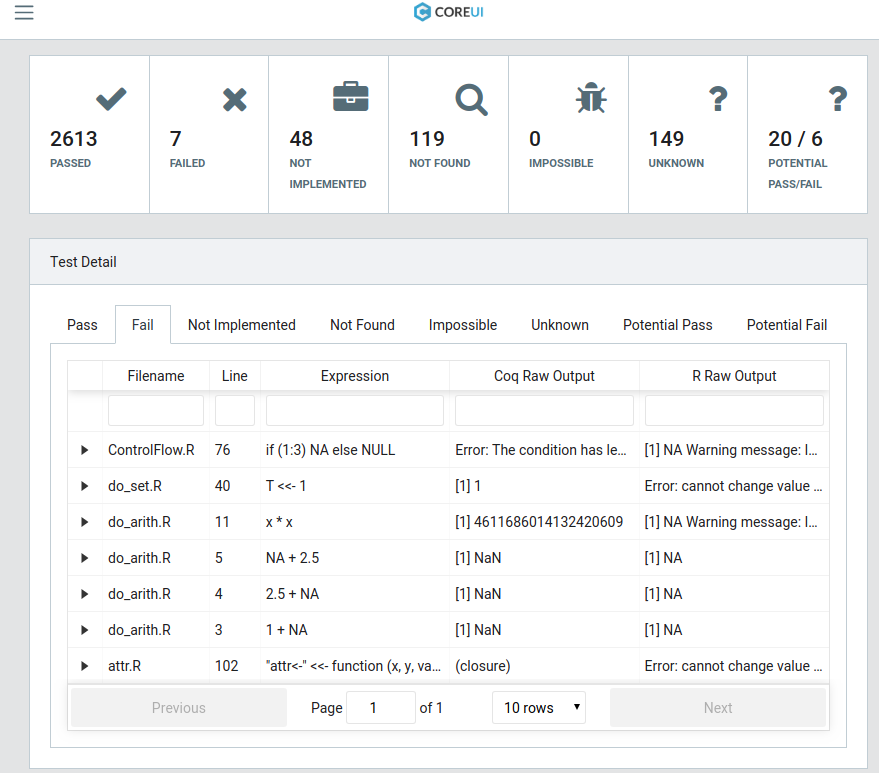
\includegraphics[width=10cm]{images/fail.png}
    \end{center}
\end{frame}

\frame{\questiontoc}

\begin{frame}
    \label{frame:full:results}
    \frametitle{Full results}

\begin{tabular}{|l||r|r|r|r|r|r|r|r|}
\hline
{\bf Suite}  & {\bf P} & {\bf F} & {\bf NI} & {\bf NF} & {\bf I} & {\bf U} & {\bf PP} & {\bf PF} \\ \hline\hline
Corners     & 2,613 & 7     & 48     &   119    & 0   & 149    &   20  & 6 \\ \hline
GNU~R       & 243   & 31    & 739    &   723    & 1   & 27     &   0   & 0 \\ \hline
FastR1      & 1,103 & 25    & 987    &   115    & 0   & 161    &   59  & 326 \\ \hline
FastR2      & 2,411 & 1,128 & 6,888  &   493    & 0   & 1,914  &   297 & 343 \\ \hline\hline
{\bf Total} & 6,370 & 1,191 & 8,662  &   1,450  &  1  & 2,251  &   376 & 675 \\
\hline
\end{tabular}

{\em total number of tests:} 20,976

\end{frame}

\frame{\questiontoc}

\frame{\tableofcontents}

\end{document}

